% !TEX root = main.tex

As predicted yesterday, the errors in the spectral method are mathematical, not computational.
Specifically, this use of the spectral method does not account for the boundary conditions of the system.
Because the system has only advection to the right, the inflow of the equations is not accounted for, and was causing substantial numerical errors. 
5 solutions were proposed, each involved in ensuring that the solution at left-most chebyshev point remains zero throughout the advection.
\begin{enumerate}
	\item Set last row and last column of differentiation matrix to zero.
	\item Compute necessary powers of differentiation matrix, then set last row and last column to zero.
	Investigation has shown this to be equivalent to method 1.
	\item Removing the last row and column of differentiation matrix.
	\item Removing last row and column of the matrix operator applied to $\hat{\vec{Q}^n}$ at every timestep, either before or after inversion.
	\item Setting the last row of the above matrix to zero before or after inversion.
\end{enumerate}
The module $\texttt{beuler\_advection.py}$ contains the framework in which we are testing the above methods.
Additionally, the code has been refactored into the function $\texttt{advection}$ which has the following declaration:
$$\texttt{q, s = def advection( tf, N, dt, q0, domain=[-1, 1], ord=2, plot=True )}$$
where \texttt{tf} is the final time at which the solution is calculated, \texttt{N} is the number of spatial discretization points, \texttt{dt} is the time-step used, \texttt{q0} is a function representing the initial condition, and \texttt{ord} is the order used in the solution.
\texttt{q} is the solution at time \texttt{tf} located at each of the chebyshev points in \texttt{s}. 
Presently, only the order 1, 2, and 3 solutions are speculated to work, although this is not certain.
The reason for this uncertainty comes from uncertainty in the choice of solution to the boundary issue.
Among the above solutions, none works exactly for higher order methods, with coarser time discretization.
This is seen in the below figure, particularly for the 5-th order method.
The exact matrices used for the higher order implicit methods are discussed below.
\begin{figure}[H]
	\centering
	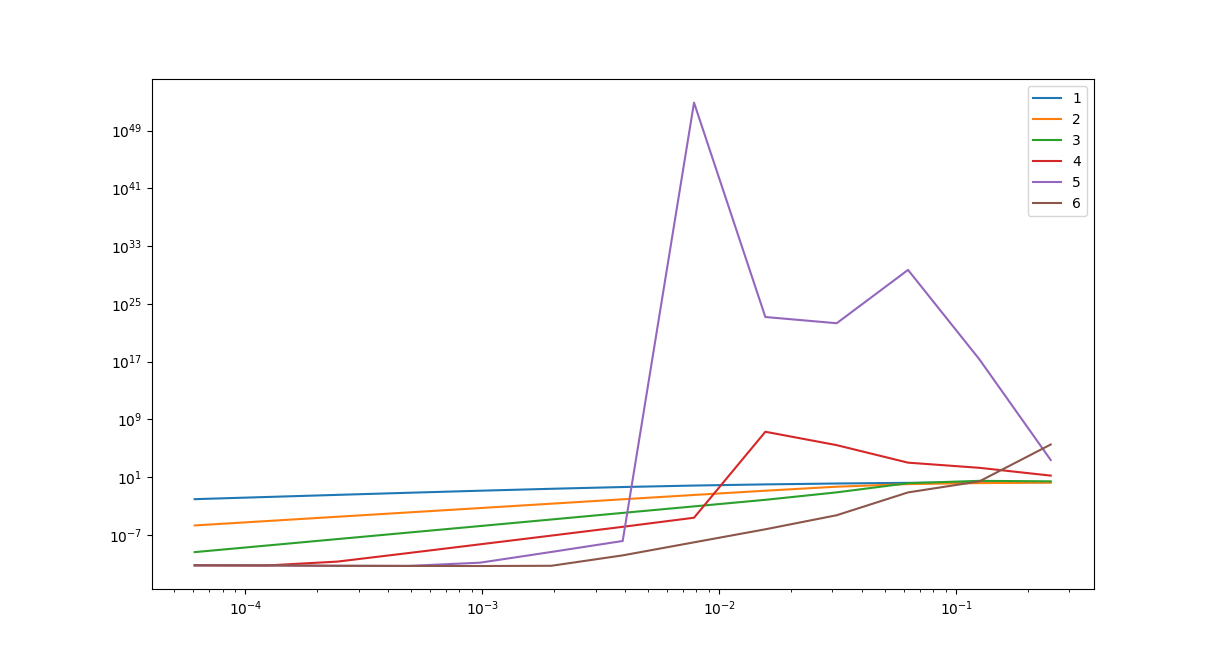
\includegraphics[width=0.5\textwidth]{bad_order_rates.png}
\end{figure}
Method 4 and 5 are presently the most underexlplored, and additional work will go into their assessment. 
Additionally, to assist in numerical stability, when high powers of the differentiation matrix are computed, the timestep is multiplied into each before exponentiation.